\documentclass{beamer}

\usepackage[utf8]{inputenc}
\renewcommand{\v}{\mathbf}


%Information to be included in the title page:
\title{Lattice-based Cryptography and LWE}
\author{Ben Young}
\institute{MATH 408}
\date{April 26, 2020}

\begin{document}

\frame{\titlepage}

\begin{frame}
\frametitle{Lattices - overview}
\begin{block}{Definition: Lattice}
    Let $\v{b}_1,\cdots,\v{b}_n \in \mathbb{R}^n$ be $n$ linearly independent vectors. 
    A \textit{lattice} $\mathcal{L}$ is defined as
\begin{equation*}
    \mathcal{L}(\v{b}_1,\cdots,\v{b}_n) = \left\{\sum_{i=1}^n{x_i\v{b}_i : x_i \in \mathbb{Z}}\right\}
\end{equation*}
\end{block}
\begin{figure}[h!]
    \caption{An example of a 2-dimensional lattice with basis vectors [1]}
    \centering
    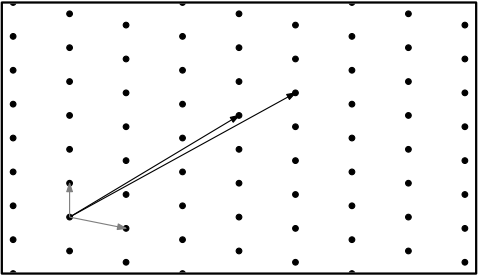
\includegraphics[scale=0.3]{lattice.png}
\end{figure}
\end{frame}

\begin{frame}
\frametitle{Lattices - overview}
We usually represent the basis as a matrix 
\begin{equation*}
    \v{B} = [\v{b_1}, \cdots, \v{b_n}] \in \mathbb{R}^{n \times n}
\end{equation*}
so that the lattice generated by $\v{B}$ is
\begin{equation*}
    \mathcal{L}(\v{B}) = \{\v{Bx}: \v{x} \in \mathbb{Z}^n\}.
\end{equation*}
\begin{block}{Definition: q-ary lattice}
A \textit{q-ary lattice} is a lattice whose
member vectors $\v{v}$ are determined component-wise mod $q$:
$q\mathbb{Z}^n \subset \mathcal{L} \subset \mathbb{Z}^n$
\end{block}
\end{frame}

\begin{frame}
\frametitle{Lattices - overview}
A way to generate a q-ary lattice from a non-square matrix:
\begin{block}{Definition: $\Lambda_q$}
Given $\v{A} \in \mathbb{Z}_q^{n \times m}$, define
\begin{equation*}
    \Lambda_q(\v{A}) := \{\v{x} \in \mathbb{Z}^m: \v{x} = \v{A}^T\v{s}
        \pmod{q} \text{ for some } \v{s} \in \mathbb{Z}^n
    \}
\end{equation*}
(lattice generated by the rows of $\v{A}$)
\end{block}
\begin{block}{Example}
\begin{equation*}
    \v{A} = \begin{bmatrix} 2 & 0 & 2 \\ 1 & 4 & 3 \end{bmatrix}, q=5
\end{equation*}
\begin{equation*}
    \begin{bmatrix}2 & 1 \\ 0 & 4 \\ 2 & 3\end{bmatrix}
    \begin{bmatrix}1 \\ 2 \end{bmatrix} \pmod{5} =
    \begin{bmatrix}4 \\ 3 \\ 3\end{bmatrix} \in \Lambda_5(\v{A})
\end{equation*}
\end{block}
\end{frame}
\begin{frame}
\frametitle{Lattices - overview}
Another way to generate a q-ary lattice from a non-square matrix:
\begin{block}{Definition: $\Lambda_q^\perp$}
Given $\v{A} \in \mathbb{Z}_q^{n \times m}$, define
\begin{equation*}
    \Lambda_q^\perp(\v{A}) := \{\v{x} \in \mathbb{Z}^m: \v{Ax} = \v{0}
        \pmod{q}
    \}
\end{equation*}
(all vectors orthogonal mod $q$ to the rows of $\v{A}$, equivalently
a code whose parity check matrix is $\v{A}$)
\end{block}
\begin{block}{Example}
\begin{equation*}
    \v{A} = \begin{bmatrix} 2 & 0 & 2 \\ 1 & 4 & 3 \end{bmatrix}, q=5
\end{equation*}
\begin{equation*}
    \begin{bmatrix} 2 & 0 & 2 \\ 1 & 4 & 3 \end{bmatrix}
    \begin{bmatrix} 3 \\ 4 \\ 2 \end{bmatrix}
    = \begin{bmatrix} 0 \\ 0 \end{bmatrix} \pmod{5}
    \text{ so } \begin{bmatrix} 3 \\ 4 \\ 2 \end{bmatrix} \in 
    \Lambda_5^\perp(\v{A})
\end{equation*}
\end{block}
\end{frame}

\begin{frame}
\frametitle{Lattice Problems}
\begin{block}{Shortest Vector Problem (SVP)}
Given a basis $\v{B}$ and approximation factor $\gamma$, find a vector 
$\v{x}$ such that $||\v{x}|| \leq \gamma||\v{s}||$, where $\v{s}$ is
the shortest nonzero vector in $\mathcal{L}(\v{B})$.
\end{block}
\begin{columns}
\column{0.4\textwidth}
\[
    \v{B} = \begin{bmatrix}13 & 7 \\ -5 & 8 \end{bmatrix},
    \gamma = 1
\]
The shortest vector in $\mathcal{L}(\v{B})$ is
\[
    \v{s} = \begin{bmatrix} 7 \\ 8 \end{bmatrix}.
\]
\textit{GapSVP} is the decision variant of SVP.
\column{0.6\textwidth}
\begin{figure}
    \includegraphics[scale=0.31]{shortest.png}
\end{figure}
\end{columns}
\end{frame}

\begin{frame}
\frametitle{Lattice Problems}
\begin{block}{Closest Vector Problem (CVP)}
    Given a basis $\v{B}$, approximation factor $\gamma$ and 
    $\v{t} \notin \mathcal{L}(\v{B})$, find a point in 
    $\mathcal{L}(\v{B})$ within $\gamma d$ of $\v{t}$,
    where $d$ is the shortest distance between any $\v{x} \in 
    \mathcal{L}(\v{B})$ and $\v{t}$.
\end{block}
\begin{columns}
\column{0.45\textwidth}
\begin{align*}
    &\v{B} = \begin{bmatrix}13 & 7 \\ -5 & 8 \end{bmatrix}, \\
    \v{t} = &\begin{bmatrix} -8, -3 \end{bmatrix},\ 
    \gamma = 1
\end{align*}
The vector in $\mathcal{L}(\v{B})$ closest to $\v{t}$ is
\[
    \begin{bmatrix} -7 \\ -8 \end{bmatrix}
\]
\column{0.55\textwidth}
\begin{figure}
    \includegraphics[scale=0.3]{closest.png}
\end{figure}
\end{columns}
\end{frame}

\begin{frame}
\frametitle{Lattice Problems}
SVP can be reduced to CVP. Let $\v{B} = [\v{b}_1, \ldots, \v{b}_n]$
be a basis. Then for $i = 1,\ldots,n$, solve CVP for basis
$\v{B}_i=[\v{b}_1,\ldots,2\v{b}_i,\ldots,\v{b}_n]$ and $\v{b}_i$,
which is not $\in \mathcal{L}(\v{B}_i)$ because $[\v{b}_1, \ldots, \v{b}_n]$ are linearly independent. Let $\v{v}_i$ be the output of CVP (the vector in 
$\mathcal{L}(\v{B}_i)$ closest to $\v{b}_i$). Then
\[
    \arg\min_{\v{v}_1-\v{b}_1,\ldots,\v{v}_n-\v{b}_n}{\|\v{v}_i-\v{b}_i\|}
\]
is the solution to SVP for $\v{B}$.
\end{frame}
\begin{frame}
\frametitle{Lattice Problems}
\begin{block}{Shortest Independent Vector Problem (SIVP)}
    Given $\v{B}$ and approximation factor $\gamma$, find $n$ linearly 
    independent lattice vectors $\{\v{x}_1, \cdots, \v{x}_n\} \subseteq
    \mathcal{L}(\v{B})$ such that $\max_i{||\v{x}_i||} \leq \gamma S$,
    where $S = \max_i{||\v{x}_i||}$ for the set of $n$ linearly independent
    vectors $\{\v{x}_1,\cdots,\v{x}_n\}$ giving the smallest such quantity $S$ 
\end{block}
\begin{columns}
\column{0.45\textwidth}
\[
    \v{B} = \begin{bmatrix}15 & 7 \\ -5 & 8 \end{bmatrix},\ 
    \gamma = 1
\]
Find the set of 2 linearly independent vectors with the shortest
longer vector. In this case it's just the two shortest unique
vectors in the lattice,
\[
    \begin{bmatrix} 7 \\ 8 \end{bmatrix}
    \text{ and }
    \begin{bmatrix} 8 \\ -13 \end{bmatrix}
\]
\column{0.55\textwidth}
\begin{figure}
    \includegraphics[scale=0.29]{independent.png}
\end{figure}
\end{columns}
\end{frame}

\begin{frame}
\frametitle{Lattice Problems}
Lattice problems are hard:
\begin{block}{Conjecture}
    No polynomial time algorithm can solve SVP, GapSVP, CVP, or SIVP to within a polynomial factor $\gamma$ [1]
\end{block}
\begin{block}{Conjecture}
    No polynomial time quantum algorithm can solve SVP, GapSVP, CVP, or SIVP to within a polynomial factor $\gamma$ [1]
\end{block}
\end{frame}

\begin{frame}
    \frametitle{Learning Problems}
    \begin{block}{Learning from parity with errors}
        Given a set of \textit{equations with errors}
    \begin{align*}
        &\v{s}\cdot \v{a}_1 \approx_\epsilon b_1 \pmod{2} \\
        &\v{s}\cdot \v{a}_2 \approx_\epsilon b_2 \pmod{2} \\
        \vdots
    \end{align*}
    where $b_i \in \mathbb{Z}_2$, the elements of each $\v{a}_i \in \mathbb{Z}^n_2$
    are sampled independently from the uniform distribution on $\mathbb{Z}_2$
    and each equation is correct with probability $1-\epsilon$,
    determine $\v{s} \in \mathbb{Z}^n_2$.
    \bigskip \\
    Easy via Gaussian elimination ($n$ unknowns $s_1,\ldots s_n$, $O(n)$ equations) 
    if $\epsilon = 0$ (all equalities guaranteed to hold) but hard
    when $\epsilon > 0$: Best known algorithm runs in time $2^{O(n/\log{n)}}$
    \end{block}
\end{frame}

\begin{frame}
\frametitle{Learning Problems}
\begin{block}{Learning with Errors (LWE)}
    Extention of learning from parity. Given prime $p$, probability distribution 
    $\chi: \mathbb{Z}_p \to [0,1]$, set of equations with error
    \begin{align*}
        &\v{s} \cdot \v{a}_1 \equiv_\chi b_1 \pmod{p} \\
        &\v{s} \cdot \v{a}_2 \equiv_\chi b_2 \pmod{p} \\
        \vdots
    \end{align*}
    $\v{a}_i$ chosen independently from uniform distribution on $\mathbb{Z}_p^n$, $b_i \in \mathbb{Z}_p$. Each $b_i = \v{s}\cdot\v{a}_i + e_i$
    where $e_i \in \mathbb{Z}_p$ is independently sampled from $\chi$.
    $\text{LWE}_{p,\chi}$ is the problem of determining $\v{s}$.
    \bigskip \\
    Learning from parity is a special case of $\text{LWE}_{p,\chi}$
    where $p=2$, $\chi(0) = 1-\epsilon$, and $\chi(1) = \epsilon$
\end{block}
\end{frame}
    
\begin{frame}
\frametitle{Learning Problems}
$\chi$ in LWE is usually a `rounded normal' distribution
$\Psi_\alpha: \mathbb{Z}_q \to [0,1]$ defined as a normal
distribution on $\mathbb{Z}_q$ centered at 0 with standard
deviation $\frac{\alpha q}{\sqrt{2\pi}}$ and rounded to the
nearest integer $\pmod{q}$.
\begin{figure}[h!]
    \caption{$\Psi_\alpha$ for $\alpha=3, q=23$, 100000 samples}
    \centering
    \includegraphics[scale=0.4]{chi.png}
\end{figure}
\end{frame}

\begin{frame}
\frametitle{Learning Problems}
Solving LWE is equivalent to decoding a random linear code.
Suppose LWE problem has $m$ equations, let 
\[
    \v{Q} = [\v{a}_1,\ldots,\v{a}_m]^T \in \mathbb{Z}^{m\times n}_p
\]
so we can reformulate the problem as recovering $\v{s}$ from
\[
    \v{b} = \v{Qs+e} \in \mathbb{Z}_p^m
\]
where each coordinate of $\v{e}$ is sampled from $\Psi_\alpha$.
The probability of sampling 0 from $\Psi_\alpha$ is roughly $\frac{1}{\alpha p}$
so the Hamming weight of $\v{e}$ (and thus the Hamming distance 
between $\v{b}$ and $\v{Qs}$) 
is roughly 
$m\left(1-\frac{1}{\alpha p}\right)$. 
For a general $\v{s}' \in \mathbb{Z}_p^n$ the expected Hamming distance
from $\v{b}$ to $\v{Qs}'$ is approximately $m\left(1-\frac{1}{p}\right)$.
So if we can solve LWE we can solve the nearest-codeword problem
to within a factor of $\frac{1-\frac{1}{p}}{1-\frac{1}{\alpha p}}$.
\end{frame}

\begin{frame}
\frametitle{Learning Problems}
\begin{block}{LWE-decision problem}
Given matrix $\v{A} \in \mathbb{Z}_p^{m \times n}$
whose elements are chosen uniformly and indepentently from $\mathbb{Z}_p$, distribution $\chi^m$ on $\mathbb{Z}_p^m$,
and a vector $\v{b}$ either (unknown to the problem solver) chosen
uniformly from $\mathbb{Z}_p^m$ or as $\v{b} = \v{A}\v{s} + \v{e}$
for uniformly chosen $\v{s} \in \mathbb{Z}_p^n$ and $\v{e} \in \mathbb{Z}_p^m$ sampled from $\chi^m$. 
Solving the problem then consists of determining
which of these two methods was used to generate $\v{b}$.
\bigskip \\
Equivalently, given $\v{a} \in \mathbb{Z}_p^n$ (a row of $\v{A}$),
distribution $\chi$ on $\mathbb{Z}_p$, and $b \in \mathbb{Z}_p$
chosen either uniformly from $\mathbb{Z}_p$ or as 
$\v{a} \cdot \v{s} + e$ for uniformly chosen $\v{s} \in \mathbb{Z}_p^n$
and $e \in \mathbb{Z}_p$ sampled from $\chi$, determine which method
was used to generate $b$.
\end{block}
\end{frame}

\begin{frame}
\frametitle{Learning Problems}
\begin{block}{Lemma}
The LWE and LWE-decision problems are equivalent. Formally,
Let $p \leq \text{poly}(n)$ be prime, $\chi$ be a probability distribution on
$\mathbb{Z}^p$. Suppose we have access to a procedure that solves the LWE-decision
problem in polynomial time for a non-negligible fraction of all possible $\v{s} \in
\mathbb{Z}_p^n$. Then we can solve $\text{LWE}_{p,\chi}$ in polynomial
time
\end{block}
\end{frame}

\begin{frame}
\frametitle{Learning Problems}
\begin{block}{Idea of proof of lemma}
    The goal is to recover $\v{s}$ from
    $\v{b} = \v{As+e}$
    where each coordinate of $\v{e}$ is sampled from $\chi$.
Recover $\v{s}$ one coordinate at a time. WLOG recover $s_1$.
Let $\v{a}_1$ be the first row of $\v{A}$ and $b_1$ be the first element of $\v{b}$.
For any $k \in \mathbb{Z}_p$, let 
\[
    T(\v{a}_1, b_1) = 
    (\v{a}_1 + [d,0,\ldots,0], b_1+lk)
    = (\v{T_a},T_b)
\]
where $d$ is uniformly chosen from
$\mathbb{Z}_p$. If $k=s_1$ then 
\begin{align*}
    T_b = b_1+dk &= b_1 + ds_1 \\
           &= \v{a\cdot s} + e_1 + ds_1  \\
    &= (\v{a}_1\cdot \v{s} + ds_1) + e_1 \\
    &= (\v{a}_1 + [d,0,\ldots,0]) \cdot \v{s} + e_1 \\
    &= \v{T_a} \cdot \v{s} + e_1
\end{align*}
\end{block}
\end{frame}

\begin{frame}
\frametitle{Learning Problems}
\begin{block}{Idea of proof of lemma (continued)}
    But if $k \neq s_1$ then since $p$ is prime and $\v{A}$
    and $d$ are sampled from the uniform distribution,
    \[
        T_b = b_1 + dk
    \]
    is also sampled from the uniform distribution.
    Thus we can use the LWE-decision oracle's answer of whether 
    $T_b = \v{T_a} \cdot \v{s} + e_1$ or $T_b$ was sampled from the 
    uniform distribution to deduce whether $k = s_1$.
    $k$ only has $p \leq \text{poly}(n)$ possible values, so we can
    check whether $s_1 = k$ for each possible value of $k$.
    We repeat this procedure $n$ times to determine each coordinate of $\v{s}$
    and thus can solve LWE in polynomial time.
\end{block}
\end{frame}

\begin{frame}
\frametitle{LWE and lattice problems}
\begin{block}{Theorem ([2])}
GapSVP and SIVP reduce to LWE-decision:

Let $n \in \mathbb{Z}$, $p \leq \text{poly}(n)$ be prime,
$\alpha \in (0,1)$ such that $\alpha p > 2 \sqrt{n}$.
Given a polynomial-time algorithm to solve $\text{LWE-decision}_{p,\Psi_\alpha}$ then there is a polynomial time quantum algorithm 
approximating GapSVP and SIVP to within $\gamma = \tilde{O}(n/\alpha)$
in the worst case.
\end{block}
\begin{block}{Corollary}
    If GapSVP and SIVP are hard (recall that we conjectured that they are)
    then LWE-decision and LWE are hard.
\end{block}
\smallskip
Rough intuition of connection between LWE-decision and lattice problems:
$\v{b} = \v{As + e}$ is equivalent to taking a random point $\v{As}$ in the
lattice $\Lambda_p(\v{A}^T)$ and slightly perturbing its coordinates
using $\Phi_\alpha$. This suggests using a CVP oracle on points
very close to $\v{As}$.
\end{frame}

\begin{frame}
\frametitle{LWE and lattice problems}
Why do we need a quantum reduction?
The reduction uses a modified oracle for CVP. Let $L$ be a lattice, 
$d$ be a distance much smaller than the length of the smallest
vector in $L$.
If $\v{x}$ is a vector within $d$ of $L$, the oracle finds the point
in $L$ closest to $\v{x}$. If $\v{x}$ is not within $d$ of $L$ then 
the oracle's output is undefined. The only way to reliably generate an input
to the oracle is to let $\v{x}=\v{y+z}$ for $\v{y} \in L$ and a
small pertubation vector $\v{z}$. Then the oracle produces $\v{y}$,
the closest vector in $L$ to $\v{x}$. But we already know $\v{y}$ since we used
it to generate $\v{x}$!

So the oracle is only useful in a quantum setting: it lets us uncompute
$\v{y}$.
\end{frame}

\begin{frame}
\frametitle{LWE and lattice problems}
So hardness of LWE depends on the \textit{quantum} hardness of
SIVP and GapSVP, a weaker condition than the \textit{classical} (non-quantum)
hardness of SIVP and GapSVP.
\bigskip \\
Peikert (2009) found a non-quantum reduction from GapSVP to LWE, so
the below LWE cryptosystem depends on the classical hardness of GapSVP.
But $p$ in the LWE problem must be exponentially large and no 
corresponding classical reduction was found for SIVP.
\end{frame}

\begin{frame}
\frametitle{LWE Cryptosystem}
[2] proposed a cryptosystem based on the conjectured hardness of the
LWE-decision problem. We present [1]'s version, which has a few
improvements.
\bigskip \\
The system has integer parameters $n$, $m$, $l$, $t$, $r$, and $q$, where $n$ is the dimension of the lattice underlying the system (and is thus
the most important security parameter), $l$ is the length of each message, and
$t$ is the size of the field over which the message bits are chosen (usually 2).
It also has real-valued parameter $\alpha > 0$, which is the spread of
the distribution $\Psi_{\alpha}$.
\bigskip \\
The system uses function $f: \mathbb{Z}_t^l \to \mathbb{Z}_q^l$ that converts
mod-$t$ vectors to mod-$q$ vectors by multiplying each coordinate in its
input by $\frac{q}{t}$ and rounding to the nearest integer.
$f$ has corresponding inverse $f^{-1}: \mathbb{Z}_q^l \to \mathbb{Z}_t^l$
that converts mod-$q$ vectors to mod-$t$ vectors by multiplying each
coordinate by $\frac{t}{q}$ and rounding to the nearest integer.
\end{frame}

\begin{frame}
\frametitle{LWE Cryptosystem}
The private key is a random uniformly-chosen matrix
$\v{S} \in \mathbb{Z}_q^{n \times l}$. 
To determine a public key, choose two more random matrices:
$\v{A} \in \mathbb{Z}_q^{m \times n}$ from a uniform distribution
and $\v{E} \in \mathbb{Z}_q^{m \times l}$ with each entry chosen
from $\Psi_{\alpha}$. Then calculate 
\begin{equation}
    \v{P} = \v{AS} + \v{E} \in \mathbb{Z}_q^{m \times l} 
\end{equation}
and the public key is the pair $(\v{A}, \v{P})$.

To encrypt a message $\v{v} \in \mathbb{Z}_t^l$ choose $\v{a} \in \{-r, -r+1, \cdots, r\}^m$ uniformly at random, calculate 
\begin{equation}
    \v{u} = \v{A}^T\v{a} \in \mathbb{Z}_q^n,\quad
    \v{c} = \v{P}^T\v{a} + f(\v{v}) \in \mathbb{Z}_q^l
\end{equation}
and send ciphertext $(\v{u}, \v{c})$.

Then to decrypt a ciphertext, calculate 
\begin{equation}
    m = f^{-1}(\v{c} - \v{S}^T\v{u}) \in \mathbb{Z}_t^l
\end{equation}
and $m$ will be the original plaintext.
\end{frame}

\begin{frame}
\frametitle{LWE Cryptosystem}
\begin{block}{Proof of security}
    \begin{itemize}
    \item
        Distinguishing between $\v{P}$ sampled uniformly and $\v{P} = \v{AS+E}$ as
    generated by the cryptosystem using $\Psi_\alpha$ entails solving LWE-decision, which is hard for certain parameter values.
    \item
    Encryption using public keys sampled from the uniform distribution (i.e. not generated
    by the cryptosystem) carries no significant information
    about the encrypted message.
\item Thus breaking the system implies the ability to distinguish between keys 
    generated by the cryptosystem and uniformly sampled keys,
    which implies the ability to solve LWE-decision.
    \end{itemize}
\end{block}
\end{frame}

\begin{frame}
\frametitle{LWE Cryptosystem}
    Improved LWE cryptosystem has better key and encrypted message sizes and fewer
    operations per encrypted bit than earlier cryptosystems
    based on hardness of lattice problems.
    \begin{itemize}
        \item Private key size $nl\log{q}$\quad ($\v{S} \in \mathbb{Z}_q^{n \times l}$)
        \item Public key size $m(n+l)\log{q}$\quad $\left((\v{A},\v{P}) \in \mathbb{Z}_q^{m \times n} \times \mathbb{Z}_q^{m \times l}\right)$
        \item Encrypted message size $(n+l)\log{q}$ \quad $\left((\v{u,c}) \in 
            \mathbb{Z}_q^n \times\mathbb{Z}_q^l\right)$
        \item $\tilde{O}\left(\frac{1}{l}m\left(l+n\right)\right)$
            operations per encrypted bit \\
            (Each $\v{v} \in \mathbb{Z}_t^l$ requires calculating
            $\v{A}^T\v{a}$ and $\v{P}^T\v{a}$ for $\v{a} \in \mathbb{Z}^m$)
        \item $\tilde{O}(n)$
            operations per decrypted bit \\
            (finding $l$-length decrypted message requires calculating
            $\v{S}^T\v{u}$ for $\v{S} \in \mathbb{Z}_q^{n \times l}$,
            $\v{u} \in \mathbb{Z}_q^n$)
    \end{itemize}
\end{frame}

\begin{frame}
    \frametitle{LWE cryptosystem implementation}
    A rough working implementation of the above cryptosystem can
    be found at
    \bigskip\\
    {\footnotesize https://github.com/the12thbenyoung/lwe\_cryptosystem/blob/master/lwe.py \par}
    \bigskip
    The rounding done by functions $f$ and $f^{-1}$
    used in the encryption and decryption procedures occasionally produces
    errors that cause the decrypted message to differ from the original plaintext.
    Thus the program uses a simple Hamming error correcting code to correct at
    most one incorrect bit per message.
\end{frame}

\begin{frame}
\frametitle{References}
\section{References}\label{sec:references}
[1] D. Micciancio and O. Regev. Lattice-based Cryptography. 2008. cims.nyu.edu/$\sim$~regev/papers/pqc.pdf
\bigskip \\
\noindent [2] O. Regev, On lattices, learning with errors, random linear codes,
and cryptography. In \textit{Proc. 37th ACM Symp. on Theory of Computing}, pages 84-93, 2005. https://cims.nyu.edu/~regev/papers/qcrypto.pdf
\bigskip \\
\noindent [3] C. Peikert, V. Vaikuntanathan, and B. Waters. A framework for
efficient and composable oblivious transfer. In \textit{Advances in
Cryptology}. Springer, 2008. https://eprint.iacr.org/2007/348.pdf
\end{frame}
\end{document}
